\section{Results}

\newcommand{\fittol}[0]{0.01~}

\begin{figure}
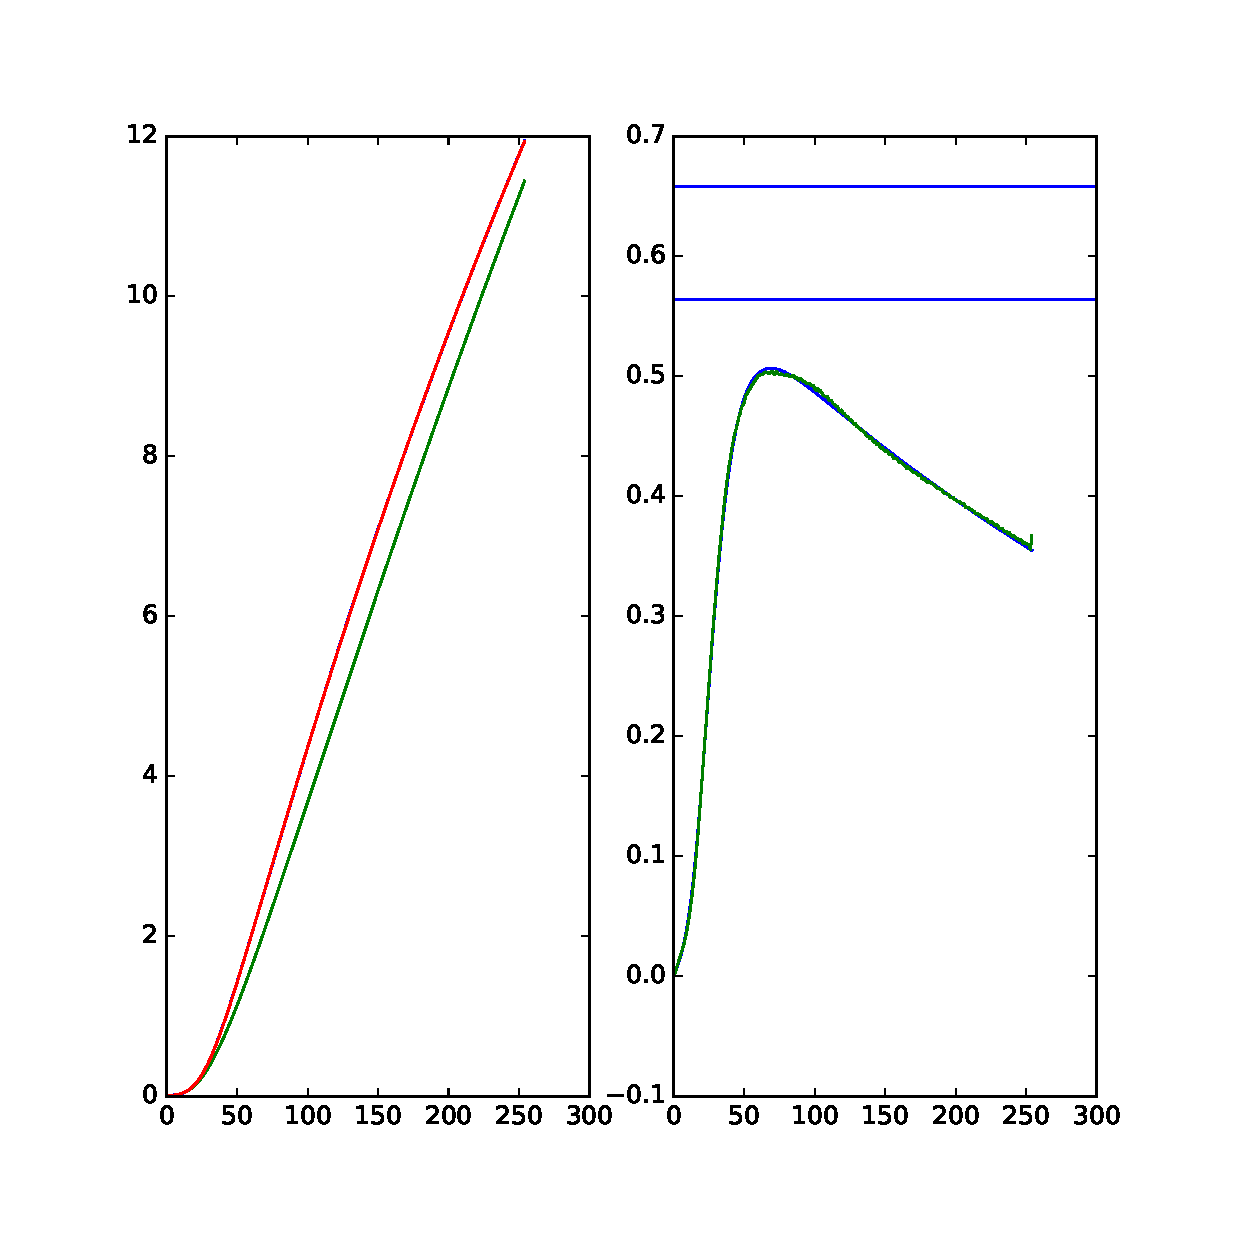
\includegraphics[width=\columnwidth]{figs/H-0.0016-0.0002.eps}
\caption{ \flabel{fit}
  Example fit.
}
\end{figure}

The numerical experiments sample the mapping from Grashof and Schmidt number to bubble height trajectory
\begin{equation*}
\left(\text{Gr}, \text{Sc}\right) \rightarrow H(t)
\end{equation*}
Each trajectory is fit to the buoyancy-drag model presented in \sref{model}, constrained by \eref{c4} and \eref{c6}, resulting in the following 4-parameter model:
\begin{align}
\ddot{h} &= \frac{A g h - C_1 \dot{h}^2 - C_2 \nu (h/\lambda) \dot{h}}{ C_3 h + \lambda/(2\pi) } \\
A &= A_0 \left[ 1 - \frac{M}{C_3 \lambda^2 h  + \lambda^3 / (2\pi)} \right]  \\
\dot{M} &= \frac{D \left[C_5 \lambda h + \lambda^2\right] ^2}{M \sqrt{\pi}} .
\end{align}
The results of the fit are a mapping from Grashof and Schmidt number to fit coefficients and root mean square error:
\begin{equation}
\left(\text{Gr}, \text{Sc}\right) \rightarrow \left(C_1, C_2, C_3, C_5, || H - h ||_2\right) 
\end{equation}

The values of the fit coefficieints, their dependence on the Grashof and Schmidt numbers, and their ability to accurately model the trajectory are the basis for the following analyses.

\subsection{Scope of model}

\begin{figure}
\includegraphics[width=\columnwidth]{figs/Err-vs-Gr-Sc}
\caption{ \flabel{errVsParam}
  Model error vs Grashof and Schmidt numbers.
}
\end{figure}

The model proposed in \sref{model} assumes the bubble is a coherent structure with a single velocity.
If the Grashof number is high, then the bubble can break up into multiple smaller bubbles as the bubble accelerates.
The break-up is easily identified visually.
Increasing the Grashof number, Schmidt number, or both should enhance the break-up, so we can identify a bifurcataion boundary for the break-up.

On the other hand, at low Grashof and Schmidt numbers, the growth of bubble height can be dominated by the growth of the interface widith, leading to predominantly diffusive dynamics.
This is particularly evident when the bubble height receeds, a process which is not accounted for in the buoyancy-drag model.
When the bubble velocity reverses, the trajectory is truncated for the purposes of fitting.
We can identify cases for which the bubble height receeds over the first time unit.
Similar to the break-up, decreasing the Grashof number, Schmidt number, or both should supress the bubble growth, so we can identify a bifurcation boundary here as well.

The accuracy of the model can be seen directly by plotting the error vs the Grashof and Schmidt numbers, as seen in \fref{errVsParam}.
The model is accurate for Rayleigh numbers above 2000.

\subsection{Fit coefficients}
The proposed model has 4 undetermined parameters.
In each case, we estimate the value a-priori by physical arguments.
Then, the estimates are used as the starting point for fitting, that is minimization of the model error over the scope of the model.

\subsubsection{Form drag coefficient, $C_1$}

\begin{figure}
\includegraphics[width=\columnwidth]{figs/C1-vs-Gr-Sc}
\caption{ \flabel{C1VsParam}
  Best fit for $C_1$ vs Grashof and Schmidt numbers.
  Cases for which the relative model error exceeds \fittol are excluded.
}
\end{figure}

The parameter $C_1$ scales the form drag and serves as a drag coefficient.  
Because we have let $C_0 = 1$, the hydralic diameter of the bubble is roughly $\lambda$.
Had we let $C_0 = 1/4$, the diameter would be the more common $\lambda/2$, but many of the parameters would be fractional.
Now, we relate $C_1$ to the drag coefficient $C_d$ in the drag equation:
\begin{equation}
C_1 \lambda^2 \dot{h}^2 = \frac{1}{2} C_d A \dot{h}^2
\end{equation}
so $C_1$ can be estimated using drag coefficients of cylindrical objects:
\begin{equation}
C_1 = \frac{1}{2} C_d \frac{A}{\lambda^2} = 0.41 \frac{A}{\lambda^2} \approx 0.3
\end{equation}

We plot the best fit values of $C_1$ vs the Grashof and Schimdt number in \fref{C1VsParam}.
$C_1$ increases with Grashof and Schmidt number.

\subsubsection{Skin drag coefficient, $C_2$}
\begin{figure}
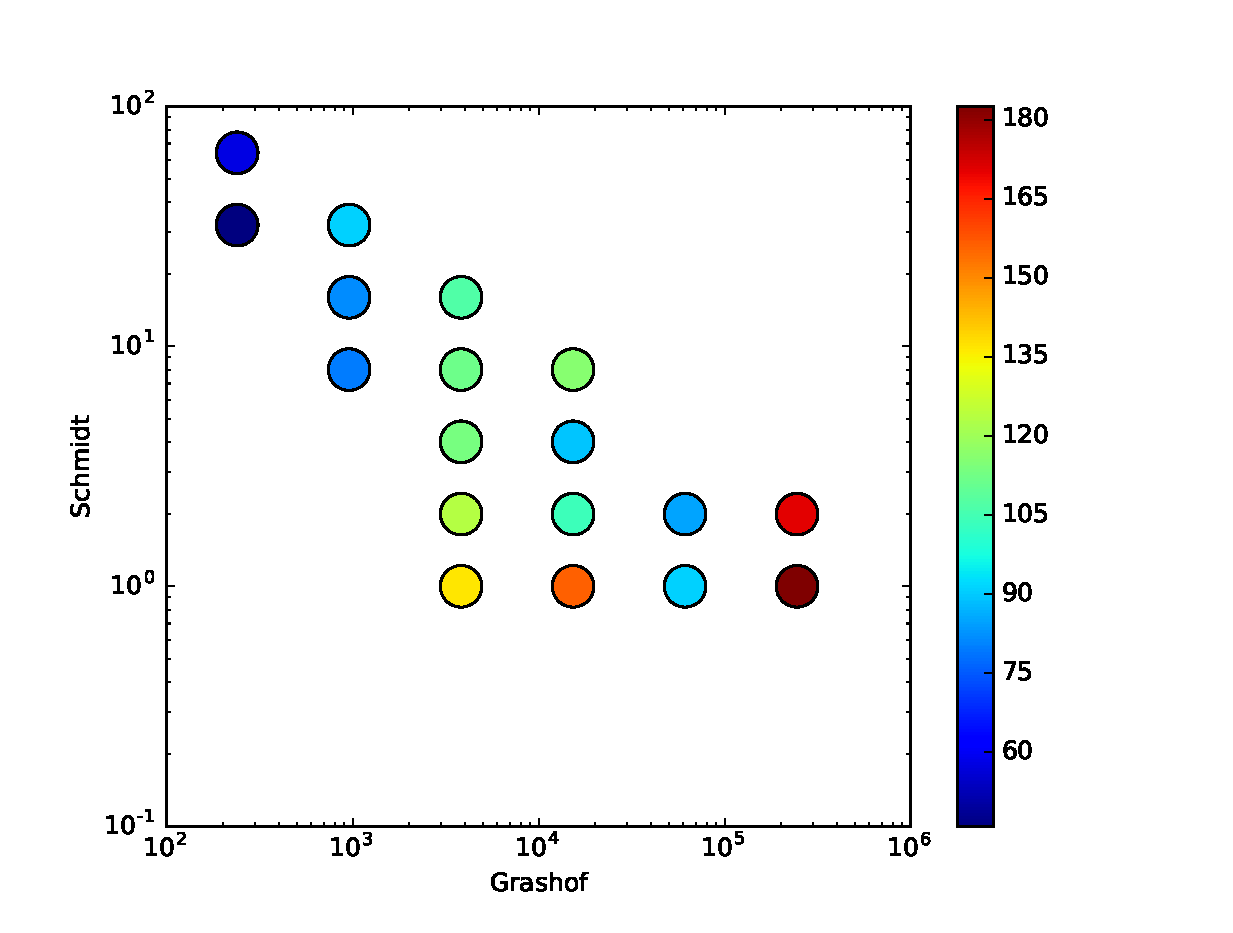
\includegraphics[width=\columnwidth]{figs/C2-vs-Gr-Sc}
\caption{ \flabel{C2VsParam}
  Best fit for $C_2$ vs Grashof and Schmidt numbers.
  Cases for which the relative model error exceeds \fittol are excluded.
}
\end{figure}

The parameter $C_2$ scales the viscous drag, so it is also a drag coefficient of sorts.
Using the analogy to Poissile flow, i.e. pipe and duct flow, we can also relate $C_2$ to the Darcy and Fanning friction factors, as in \sref{model}
\begin{equation}
\dot{h} = \frac{A g \lambda}{C_2 \nu} = \sqrt{A g \lambda^2 }
\end{equation}

\subsubsection{Inertial coefficient, $C_3$}
\begin{figure}
\includegraphics[width=\columnwidth]{figs/C3-vs-Gr-Sc}
\caption{ \flabel{C3VsParam}
  Best fit for $C_3$ vs Grashof and Schmidt numbers.
  Cases for which the relative model error exceeds \fittol are excluded.
}
\end{figure}


The parameter $C_3$ gives the ratio of the inertial height to the buoyant height.
Excepting the effects of interfacial mixing, which are accounted for seperately, the interial and buoyant heights should be the same.
In other words, entrainment of non-buoyant fluid at the head and tail of the bubble should not scale with the height.

\subsubsection{Interfacial area coefficient, $C_5$}
\begin{figure}
\includegraphics[width=\columnwidth]{figs/C5-vs-Gr-Sc}
\caption{ \flabel{C5VsParam}
  Best fit for $C_5$ vs Grashof and Schmidt numbers.
  Cases for which the relative model error exceeds \fittol are excluded.
}
\end{figure}



The parameter $C_5$ gives the ratio of the bubble height and diameter to the interfacial area.
If the bubble were a cylinder, $C_5 = \pi$; if the bubble where rectangular, $C_5 = 4$.


\subsection{Validating limits}
To validate the limits imposed by the linear theory, we repeat the fit allowing those values to change.
The result is a model error of ???, which is ???\% less than fit with the limits strictly imposed.
This small change in model accuracy indicates that model is compatible with those limits.


